\documentclass[BTech]{iitmdiss}

\usepackage[utf8]{inputenc}
\usepackage{mathtools}
\usepackage{amsthm}
\usepackage{epstopdf}
\usepackage{times}
\usepackage{epsf}
\usepackage{threeparttable}
\usepackage{setspace}
\usepackage{amsmath}
\usepackage{amsthm}
 \usepackage{amsfonts}
\usepackage{epsfig}
\usepackage{caption}
\usepackage{subfig}
\usepackage[dvips]{graphicx}
%  \usepackage[square,numbers,sort]{natbib}
\usepackage[square]{natbib}
\usepackage[hypertex]{hyperref} % hyperlinks for references.
% \usepackage{algorithmic}
\usepackage{program}
\usepackage[boxed, algochapter, boxruled]{algorithm2e}
% \usepackage{cite}


%\include{commands}

% Strut macros for skipping spaces above and below text in tables. 
\def\abovestrut#1{\rule[0in]{0in}{#1}\ignorespaces}
\def\belowstrut#1{\rule[-#1]{0in}{#1}\ignorespaces}

\def\abovespace{\abovestrut{0.20in }}
\def\aroundspace{\abovestrut{0.20in}\belowstrut{0.10in}}
\def\belowspace{\belowstrut{0.10in}}
%%%%%%%%%%%%%%%%%%%%%%%%%


\def\thesistitle{The Maximum Flow Problem in Undirected Graphs}
\def\thesisauthor{Karthik Abinav S}


\begin{document}
\bibliographystyle{ieeetr}
%%%%%%%%%%%%%%%%%%%%%%%%%%%%%%%%%%%%%%%%%%%%%%%%%%%%%%%%%%%%%%%%%%%%%% 
% Title page

\title{\thesistitle}

\author{\thesisauthor}

\date{May 2014}
\department{Computer Science and Engineering}

%\nocite{*}
\begin{singlespace}
\maketitle 
\end{singlespace} 


\newtheorem{thm}{Theorem}
\newtheorem{thm2}{Statement}
\newtheorem{lemma}{Lemma}
\newtheorem{prop}{Proposition}
\newtheorem{modif}{Modification}
\newtheorem{defn}{Definition}

%%%%%%%%%%%%%%%%%%%%%%%%%%%%%%%%%%%%%%%%%%%%%%%%%%%%%%%%%%%%%%%%%%%%%%
% Certificate
\certificate

\vspace*{0.5in}

\noindent This is to certify that the report entitled {\bf {\thesistitle}}, 
submitted by {\bf {\thesisauthor}}, to the Indian Institute of Technology, 
Madras, for the award of the degree of {\bf Bachelor of Technology}, 
is a bona fide record of the research work carried out by him under my
supervision. The contents of this report, in full or in parts, have not been
submitted to any other Institute or University for the award of any degree or
diploma.

\vspace*{1.4in}
\hspace*{-0.25in}
\begin{singlespace}
\noindent {\bf Dr.~N.~S.~Narayanaswamy } \\
\noindent Research Guide \\ 
\noindent Associate Professor \\
\noindent Dept. of Computer Science and Engineering\\
\noindent IIT-Madras, 600 036 \\
\end{singlespace}
\vspace*{0.20in}
\noindent Place: Chennai\\ 
Date:

%%%%%%%%%%%%%%%%%%%%%%%%%%%%%%%%%%%%%%%%%%%%%%%%%%%%%%%%%%%%%%%%%%%%%%
% Acknowledgements
\acknowledgements

  I would like to thank Prof. Narayanaswamy for guiding me through the course of this project and giving me pointers to various reading material
  whenever I needed them. The discussions with him during the course of project enhanced my understanding of this topic and shaped my new ideas.
  I would also like to convey my sincere gratitude to the theory professors in the department namely Prof. Jayalal Sarma, Prof. Ragavendra Rao and
  Prof. Pandu Rangan for the various courses I took with them, which helped me enhance my interest towards this subject. I would also like to thank the 
  professors in my department, whose courses gave me a solid foundation in computer science.\\
  
  I would also like to thank my parents and brother for their constant support during the ups and downs of my life. I would also like to thank 
  my wingmates and classmates for their constant encouragement and help during my years of stay here. And finally, I would also like to thank the department
  for providing an opportunity to conduct research as an undergraduate, which helped me in making an informed career choice.

%%%%%%%%%%%%%%%%%%%%%%%%%%%%%%%%%%%%%%%%%%%%%%%%%%%%%%%%%%%%%%%%%%%%%%
% Abstract

\abstract

\noindent KEYWORDS: \hspace*{0.5em} \parbox[t]{4.4in}{Graph Theory,
Maximum Flow, Laplacian Solvers }

\vspace*{24pt}

Maximum flow problem has been a very important optimization problem in computer science and mathematics. This problem has a lot of practical relevance.
Some of the age-old applications involving maximum flow have been in electrical circuits, water supply networks, etc. With the advent of social media
and social networks, this problem has found a newer practical relevance. Since the graphs in these networks are typically very large,
researchers are sought after creating faster and more efficient algorithms for this problem. \\

Some of the classical algorithms to solve this problem are the Ford-Fulkerson's augmenting path algorithm and the Edmond-Karp algorithm. These algorithms
compute the exact value of the maximum flow. It is also fairly straightforward to obtain the optimal flow vector after the termination of the
algorithm. The main drawback with this algorithm is that the running time, although polynomial, is very high and is expensive to use in many practical
situations. Following these algorithms, a series of algorithms based on push-relabel and blocking flow techniques were devised which had a slightly better running time when compared to the 
classical algorithms. The series of algorithms terminated with the algorithm by Goldberg-Rao which gave a O($\min(n^{\frac{2}{3}},m^{\frac{1}{2}}) \log(\frac{n^2}{m}) \log U$)-time algorithm
where edge capacities are from the set $\{1,2,\ldots,U\}$. For 
extremely large graphs, as in the case of social networks, this algorithm is still far from being practical. \\

In 2008, in the breakthrough result by \cite{DBLP:journals/corr/abs-0808-4134}, they gave an algorithm to solve the Symmetric Diagonally Dominant(SDD) system of equations in 
near-linear time. This work was immediately extended by \cite{DBLP:journals/corr/abs-1003-2958} where they gave an efficient algorithm to produce an incremental graph sparsifier.
Development of these techniques led to an almost linear time algorithm to the maximum flow problem by Christiano-Kelner-Madry-Spielman-Teng.
This involved looking at the graph as a resistive network, approximating the electrical flow and producing an approximate $s-t$ flow from this approximate
electrical flow. This algorithm broke the running time barrier of Golderg-Rao and gave the first almost-linear time algorithm. \\

In this report, we give a survey of the above algorithms for the maximum flow problem. We first start off by giving a brief description of the 
classical algorithms. We then conclude this by giving a completely recursive specification for the push-relabel algorithm.
We then present tools from spectral graph theory and linear algebra that is required to understand the almost linear 
time algorithm. Following this, we present the Christiano-Kelner-Madry-Spielman-Teng algorithm in detail. Finally, we give some arguments to justify the requirement of the weight updates and also show some steps that can possibly
lead to making the algorithm parallel.\\

\pagebreak
% \listoftables
% \addcontentsline{toc}{chapter}{LIST OF TABLES}
% \listoffigures


%%%%%%%%%%%%%%%%%%%%%%%%%%%%%%%%%%%%%%%%%%%%%%%%%%%%%%%%%%%%%%%%%
% Table of contents etc.

\begin{singlespace}
\tableofcontents
\thispagestyle{empty}

% \listoftables
% \addcontentsline{toc}{chapter}{LIST OF TABLES}
%  \listoffigures
%  \addcontentsline{toc}{chapter}{LIST OF FIGURES}
\end{singlespace}


%%%%%%%%%%%%%%%%%%%%%%%%%%%%%%%%%%%%%%%%%%%%%%%%%%%%%%%%%%%%%%%%%%%%%%
% Abbreviations
\abbreviations
 
\noindent 
\begin{tabbing}
 xxxxxxxxxxx \= xxxxxxxxxxxxxxxxxxxxxxxxxxxxxxxxxxxxxxxxxxxxxxxx \kill
\textbf{IITM}   \> Indian Institute of Technology, Madras \\
 \textbf{LP}  \> Linear Program \\
\textbf{BFS} \> Breadth First Search \\
\textbf{DFS} \> Depth First Search \\
 \textbf{SCC} \> Strongly Connected Components \\
\textbf{SDD} \> Symmetric Diagonally Dominant \\
\textbf{CKMST} \> Christiano-Kelner-Madry-Spielman-Teng Algorithm \\
 \textbf{KMP} \> Koutis-Miller-Peng Solver \\
 \textbf{PSD Matrix} \> Positive Semi-Definite Matrix \\
\end{tabbing}

\pagebreak

%%%%%%%%%%%%%%%%%%%%%%%%%%%%%%%%%%%%%%%%%%%%%%%%%%%%%%%%%%%%%%%%%%%%%%
%Notation

 \chapter*{\centerline{NOTATION}}
 \addcontentsline{toc}{chapter}{NOTATION}
 
 \begin{singlespace}
 \begin{tabbing}
 xxxxxxxxxxx \= xxxxxxxxxxxxxxxxxxxxxxxxxxxxxxxxxxxxxxxxxxxxxxxx \kill
 \textbf{$m$}  \> The number of edges in a graph G \\
 
 \textbf{$n$} \> The number of vertices in a graph G \\
 
 \textbf{$u$}  \> An $m \ast 1$ matrix containing the capacities of the edges \\
 
 \textbf{$r$}  \> An $m \ast 1$ matrix containing the resistances of the links in the network \\
 
 \textbf{$U$}  \> This defines the ratio between the highest and lowest capacity in the graph, i.e.\\
		  \hspace{25mm}$\frac{\displaystyle\max_e u_e}{\displaystyle\min_e u_e}$ \\
 \textbf{$R$}  \> This defines the ratio between the highest and lowest resistance in an electrical network, i.e.\\
		  \hspace{25mm}$\frac{\displaystyle\max_e r_e}{\displaystyle\min_e r_e}$ \\
 \textbf{$A^{-1}$} \> $A^{-1} = (A^{T}.A)^{-1}.A^{T}$ (psuedo inverse) whenever A is a rectangular matrix. \\
 \textbf{$\| x \| _Q$} \> Norm with respect to the positive semi-definite matrix Q is defined as $\sqrt{x^T Q x}$ \\
 
 \end{tabbing}
 \end{singlespace}
 
 \pagebreak
 \clearpage

%The main text will follow from this point so set the page numbering
%to arabic from here on.
\pagenumbering{arabic}


%%%%%%%%%%%%%%%%%%%%%%%%%%%%%%%%%%%%%%%%%%%%%%%%%%
% Introduction.

 \chapter{INTRODUCTION}
 \label{chap:intro}
    Maximum-Flow problem is an age old optimization problem in mathematics and computer science. Hundreds of researchers have investigated this problem
    and have given some interesting results. This problem has far-reaching applications in almost every field of engineering and science. Hence, this 
    problem is of great importance, not just theoretically, but also in real-world applications. Devising better and more efficient algorithms
    for this problem and its variants, has always been the pursuit. Inspite of having had lots of research into this problem, we were far from getting an algorithm
    that has a running time suitable for practical purposes. This gives an indication of the hardness of this problem.
    
    \section{Basics}
      \subsubsection{Graph}
      A \textit{graph} G($V$, $E$, $\rho$) is defined as a mathematical structure on the set of vertices $V$ and the set of edges $E$ and an adjacency
      function $\rho : V \times V \rightarrow E$, such that $\rho(a,b) = e$ for $a,b \in V$ and $e \in E$ tells that there exists an edge $e$ between 
      the vertices $a$ and $b$.
      
      \subsubsection{Undirected Graph}
	An \textit{undirected graph} is a graph where the function $\rho$ is symmetric, i.e. $\rho(a,b) = \rho(b,a)$.
 
      \subsubsection{Directed Graph}
	A \textit{directed graph} is a graph where the function $\rho$ is not necessarily a symmetric function.
	
      \subsubsection{Capacitated Graph}
	A \textit{capacitated graph} is a graph defined as G($V$, $E$, $\rho$, $\psi$), where the first three values in the tuple mean the same as before.
	The $\psi$ in the definition is a function $\psi: E \rightarrow \mathbb{R}$, which assigns a real number corresponding to every edge $e$ in the 
	graph. This real number is called the \textit{capacity} of the graph.
      
      \subsubsection{s-t Flow}
	A \textit{s-t flow} is a vector $f \in \mathbb{R}^{\mid E \mid}$ such that the following two criteria hold:
	\begin{itemize}
	 \item 
	   Flow Conservation: $$\displaystyle\sum_{e \in E^+(v)} f(e)- \displaystyle\sum_{e \in E^-(v)} f(e) = 0 ~~~~~ \forall v \in V \setminus \{s,t\}$$
	   where $E^-(v)$ denotes the set $\{a: \rho(a,v) \text{ is defined}\}$ and $E^+(v)$ denotes the set $\{a: \rho(v,a) \text{ is defined}\}$ \\
	   
	   In an undirected graph, an arbitrary direction can be interpreted to get $E^+$ and $E^-$. For example, if the coordinate in the flow vector is
	   positive, it can be interpreted as flow entering a vertex and if the coordinate is negative, it can be interpreted as flow leaving a vertex.
	   
	 \item
	  Capacity maintenance:
	    $$f(e) \leq \psi(e)~~~~~\forall e \in E$$
	      
	\end{itemize}
	
	Additionally, the \textit{value} of the flow $f$ is a real number $F$ such that,
	$$\mid f\mid  = F = \displaystyle\sum_{e \in E^+(s)} f(e)- \displaystyle\sum_{e \in E^-(s)} f(e)$$
	
      \subsubsection{s-t Cut}
	A \textit{s-t cut} is defined as a partition of the vertex set $V$ into $U_1$ and $U_2$ such that, $s \in U_1$ and $t \in U_2$ and the vertices
	in $V \setminus \{U_1, U_2 \}$ is present exactly in one of $U_1$ and $U_2$.
      
      \subsubsection{Minimum s-t Cut Problem}
	Given a weighted graph G, let $\phi(\{U_1,U_2\})$ denote the sum of weights of edges such that one of its endpoints is in $U_1$ and the other
	end point is in $U_2$. The \textit{minimum s-t cut problem} is to select that cut, among all possible s-t cuts, whose value of $\phi$ is minimized.
      \section{Maximum Flow Problem}
	Given a capacitated graph G($V$, $E$, $\rho$, $\psi$), a source vertex s and a sink vertex t, the goal of the problem is to find the s-t flow
	such that, the value of the flow is maximized among all possible s-t flows. \\
	
	\subsection{Simple Linear Program Definition}
	  This problem can be posed as a linear programming problem. The first observation is that since LP's are efficiently solvable in polynomial
	  time, this will give us a polynomial time algorithm. The dual to the linear
	  program has a specific interpretation in graph theory. Hence, one can devise potentially more faster algorithms by using primal-dual
	  methods.
	  
	  $$\max \displaystyle\sum_{u:(s,u) \in E} f((s,u))$$
	  subject to
	  \begin{itemize}
	   \item
	      $\forall v \in V \setminus \{s,t\}$ $\displaystyle\sum_{(u,v) \in E} f((u,v))$ = $\displaystyle\sum_{(v,w) \in E} f((v,w))$
	   \item
	      $\forall (u,v) \in E$, $f((u,v)) \leq c((u,v))$
	   \item
	      $\forall(u,v) \in E$, $f((u,v)) \geq 0$
	      
	  \end{itemize}
	  
	  Note that a tuple (a, b) represents an edge e whose end points are a and b. \\
	  
	  Clearly, the vector $f \in \mathbb{R}^{\mid E\mid }$ forms the set of variables in this LP. The constraints are given to ensure that the set of 
	  solutions are the set of valid s-t flows. There is a constraint on the flow conservation on f and the capacity maintenance on f. Hence, for the
	  given problem instance, the number of variables are polynomial in $\mid E\mid $ and $\mid V\mid $ and the number of constraints are also polynomial in $\mid E\mid $
	  and $\mid V\mid $. \\
	  
	  Sometimes, an alternative formulation of the LP is given for this problem.\\
	  
	  $f$ is a vector from $\mathbb{R}^{\mid P\mid }$, where $\mid P\mid $ is the number of s-t paths in the graph. $F$ is a vector from $\mathbb{R}^{\mid V\mid }$
	  and $\gamma$ is a vector from $\mathbb{R}^{\mid E\mid }$. $f(i)$ denotes the flow that goes through the path $i$. $F(v)$ denotes the flow that 
	  is accumulated in the vertex v and $\gamma((i,j))$ denotes the flow that flows through the edge $(i,j)$. \\
	  
	  
	  $$ \max \displaystyle\sum_{i \in P} f(i) $$
	  subject to:
	  
	  \begin{itemize}
	   \item 
	      $\forall i \in P$
	      $$\forall (j,k) \in i,~~~f((j,k)) \leq c((j,k))$$
	   
	   \item
	      $f \succeq 0$
	  \end{itemize}
	  
	  
	  
	  Clearly, the number of variables and the number of constraints are both exponential. Hence, we can't really hope to solve this in polynomial
	  time. The only advantage of this formulation is that an optimal solution to this LP helps one visualize the amount of flow that goes through
	  each path independently. This formulation helps in the understanding of some of the path augmenting algorithms.
	
	\subsection{Dual of the Maximum Flow LP}
	  The dual to the maximum flow LP has a very interesting connection to graph theory. In fact, as observed ahead, the dual is a relaxation 
	  to the \textit{Minimum Cut Problem}. This is the dual corresponding to the initial primal formulation.\\
	  
	  $$\min \displaystyle\sum_{(u,v) \in E} c((u,v)) \ast y((u,v))$$
	  
	  subject to:
	  \begin{itemize}
	   \item 
	    $\displaystyle \sum_{(u,v) \in p} y((u,v)) \geq 1~~~~~~\forall p \in P$
	   \item
	    $y((u,v)) \geq 0 ~~~~~~~~~~ \forall (u,v) \in E$
	   
	  \end{itemize}

	  Here, $y$ is the dual vector corresponding to the constraints in the primal; hence, $y \in \mathbb{R}^{\mid E\mid }$.  $P$ is the set of all
	  s-t paths in the graph. \\
	  
	  From the constraints, we can now interpret the dual as the relaxation to the s-t minimum cut problem. The vector y can be interpreted 
	  as the weight assigned to each edge in the graph. For every s-t path, the sum of edge weights in that path should be atleast one. And the 
	  objective is to minimize the weighted sum of these edge weights given by the vector $y$. Hence, one optimal solution to this above LP
	  will consist of assigning a weight of 1 to the edge with minimum $c$ in every s-t path and 0 to the other edges. This, in fact, gives the 
	  value of the minimum s-t cut in the graph and the edge with weights 1 forms the edge across the cut. \\
	  
	  Now, consider the following randomized rounding procedure to find a cut $(U_1, U_2)$ such that $\phi((U_1, U_2)) \leq OBJ$ where OBJ is 
	  the value of the objective for the dual, for a given vector $y$. \\
	  
	  Let the values given by the vector $y$ be weights of the edge. Now, consider any shortest path from s to v, and let d(v) be that 
	  shortest distance for vertex v. Choose a value of $h$ uniformly at random from $[0,1)$. Consider the set 
	  $R = \{v:d(v) \leq h\}$. Clearly, from the constraints above, corresponding to any feasible solution to the dual, $t$ will not be contained 
	  in the set $R$ and $s$ will be contained in the set $R$. Hence, $R$ forms a valid s-t cut. \\
	  
	  From linearity of expectation, we get
	  $$\mathbb{E}[\phi(R)] = \displaystyle\sum_{(i,j) \in E} c((i,j)) \mathbb{P}[i \in R \wedge j \notin R]$$
	  $$\mathbb{P}[i \in R \wedge j \notin R] = \mathbb{P}[d(i) \leq h < d(j)] = d(j)-d(i)$$
	  Also, from triangle inequality note that 
	  $$d(j) \leq d(i) + y((i,j))$$
	  
	  Hence, $\mathbb{E}[\phi(R)] \leq OBJ$ and therefore, there exists a cut $(U_1,U_2)$, such that $\phi((U_1, U_2)) \leq OBJ$. \\
	  
	  Hence, the dual to the maximum flow problem is a relaxation of the s-t minimum cut problem.


	 \chapter{Classical Algorithms}
	  In this chapter, we describe some of the classical algorithms to find the exact value of the maximum flow in an undirected graph. These
	  algorithms have been widely used and give lot of insight into the problem. 
	  
	  \section{Ford-Fulkerson Augmenting Path Algorithm}
	    This is the probably the most widely known algorithm for this problem. This algorithm falls into the class of primal-dual algorithms.
	    

	    \begin{algorithm}[H]

% 	      \BEGIN \\ %
		\For{every edge (i,j) $\in$ E}{
		  Initialize f((i,j)) = 0\;
		}
 		\While{$\exists$ a path p from s to t in the residual network $G_f$}{ 
 		    $c_f(p) = \min\{c_f((i,j)): (i,j) \in p\}$ \;
 		    \For{each edge (i,j) $\in$ p}{
			\eIf{(i,j) $\in$ E}{ 
			  f((i,j)) = f((i,j)) + $c_f(p)$\;
			}
			{
 				f((i,j)) = f((i,j)) - $c_f$(p)\;	
			}

		    }
		}
		\caption{Ford-Fulkerson algorithm to compute the maximum flow}
	    \end{algorithm}
	    
	    The running time of this algorithm mostly depends on the augmentation method used to obtain the residual network. We can show that 
	    for a suitably chosen ``ill set'' of edge capacities, the number of iterations taken by the above algorithm can be very large, if the augmenting
	    paths are not chosen carefully. Edmond-Karp algorithm precisely solves this part by choosing the shortest augmenting path in each iteration
	    and hence, bounding the overall running time to $O(V E^2)$.
	  
	  \section{Edmond-Karp Algorithm}
	    This algorithm is almost identical to the Ford-Fulkerson algorithm, except for the fact that it chooses the shortest augmenting path using 
	    a Breadth-First search.
	    
	    \begin{algorithm}[H]
	      
	      
		\For{every edge (i,j) $\in$ E}{
		  Initialize f((i,j)) = 0 \;
		}
		
		\While{$\exists$ a \textbf{shortest unweighted path p} from s to t in the residual network $G_f$}{
		    $c_f(p) = \min\{c_f((i,j)): (i,j) \in p\}$\;
		    \For{each edge (i,j) $\in$ p}{
		      \eIf{(i,j) $\in$ E}{
		      
			f((i,j)) = f((i,j)) + $c_f$(p)\;
		      }
		      {
			f((i,j)) = f((i,j)) - $c_f$(p)\;
		      }
		   } 
		}    
	      \caption{Edmond-Karp algorithm to compute the maximum flow}
	    \end{algorithm}
	    	  
	    The part of the algorithm that is in bold is the only difference between this algorithm and Ford-Fulkerson's algorithm. The advantage 
	    however is that now, the number of residual graphs generated is bounded, independent of the edge capacities. \\
	    
	    The above algorithms were the most efficient known for a long time in the literature until, Goldberg and others introduced the 
	    class of algorithms known as the push-relabel algorithms. \\
	    
	   \section{Push-Relabel Algorithms}
	      In this section, we will describe the general template of any push-relabel algorithm and present a fully recursive specification
	      of the relabel-to-front algorithm. A completely recursive specification hence, allows programmers to directly to adapt it into languages
	      such as prolog. \\
	      
	      
	      \subsubsection{Generic Template of the Push Relabel Algorithm}
	      In this section, we will describe a generic template for any push-relabel algorithm. This is adapted from the text given by 
	      \cite{clrs}.
	      
	      Associate with every vertex in the graph two parameters, namely potential and reservoir.
	      \begin{itemize}
	       \item 
		  The potential is a measure of knowing the direction in which particular flow should be sent.
	      In some sense, it is used to measure the progress of the algorithm between two iterations.
	      The flow is always sent from a vertex of higher potential to a vertex of lower potential. \\
	      
	      \item
		  The reservoir stores the excessive flow that has been sent to this vertex. Since, in this algorithm the flow conservation is maintained,
		  some flow that has already been sent to this vertex cannot be routed further ahead. Hence, this keeps track of the excessive flow 
		  that accumulates at every vertex. \\
		  
		  
	      \end{itemize}

	      
	      \begin{algorithm}[H]
	            
	      \Begin( INIT\_PREFLOW {(G,s)}: ){
		
 		\For{every vertex v $\in$ V}{
 		  potential(v) := 0 \;
 		  reservoir(v) := 0 \;
 		}
		
 		\For{each edge (i,j) $\in$ E}{
 		  f((i,j)) := 0 \;
 		}
		
 		potential(s) = n \;
		
 		\For{each vertex v $\in$ N(s)}{
 		  f((s,v)) = c((s,v)) \;
 		  reservoir(v) = c(s,v) \;
 		  reservoir(s) = reservoir(s) - c((s,v)) \;
 		}
 		\caption{Initializing the preflow}
	    }
	    
	    \end{algorithm}
	      The above procedure initializes the required variables and vectors before the start of the algorithm. \\
	      
	    \textbf{Overflowing vertex} : We say a vertex v is \textit{overflowing}, if the reservoir at vertex $v$ has positive flow accumulated in it,
	    i.e. reservoir(v) $>0$. \\
	    
	    As the name suggests, at every iteration we associate two types of operations, a push operation and the relabel operation.
	    \begin{itemize}
	     \item 
	      \textit{Push operation}: This operation is performed on vertices u and v by pushing some of the accumulated flow at u to vertex v.
	      This is applicable only when the vertex u is overflowing, $c_f((u,v))>0$ and potential(u) = potential(v) + 1. Here, $c_f$ refers to the 
	      capacities in the residual network with respect to the flow f. The operation involves pushing $\min($reservoir(u), $c_f((u,v))$) units of flow
	      from u to v.
	     \item
	      \textit{Relabel}: This operation involves re-assigning the potential of the vertex u. This is applicable only when $u$ is overflowing, and
	      $\forall v \in V$ such that $(u,v) \in E_f$, we have potential(u) $\leq$ potential(v). Here, $E_f$ = $\{(i,j) \in E : f((i,j)) < c((i,j))\}$.
	      The operation involves re-assigning the potential of this vertex u with one more than the minimum of all such $v$.
	    \end{itemize}
	    
	    \begin{algorithm}[H]
	      \Begin(PUSH{(u, v)}:)
	      {
		$\Delta_f((u,v)) = \min(\text{reservoir(u)}, c_f((u,v)))$ \;
		
		\eIf{(u,v) $\in E_f$}
		{
		    f((u,v)) = f((u,v)) + $\Delta_f((u,v))$ \;
		}
		{
		  f((v,u)) = f((v,u)) - $\Delta_f((u,v))$ \;
		}
				
		reservoir(u) = reservoir(u) - $\Delta_f((u,v))$ \;
		reservoir(v) = reservoir(v) + $\Delta_f((u,v))$ \;
	      }
      
	      \caption{Push Operation}
	    \end{algorithm}
	    
	    \begin{algorithm}[H]
	      \caption{Relabel Operation}
	      
	      \Begin(RELABEL{(u)}:){
		potential(u) =  1 + $\min \{\text{potential(v)} : (u,v) \in E_f \}$ \;
	      }
	    \end{algorithm}
	    
	    With the above two functions available, a generic push-relabel algorithm looks as follows:
	    
	    \begin{algorithm}[H]
	      \caption{Push Relabel Template}
	      
	      \Begin(MAX-FLOW{(G, s, t)}:)
	      {
		INIT\_FLOW(G, s) \;
		\While{$\exists$ an applicable push or relabel operation}{
		   Call the appropriate push or relabel operation \; 
		}
	      }
	    \end{algorithm}

	    The proof of correctness of this algorithm can be shown by using the potential function on the vertices. We omit the proof here. The 
	    reader is encouraged to read \cite{clrs} for more details. \\
	    	    
	    Based on the specific implementation of the template i.e. the order of push and relabel operations performed, we can bound the running time 
	    of the algorithm. In the following sub-section, we give a fully recursive specification of the relabel-to-front algorithm and bound the 
	    running time of this algorithm. \\
	    
	    We will need the following definitions before describing the algorithm.
	    
	    \begin{defn}[\textbf{Delta indicator}]
	      A vector $L$, which is a delta indicator for a particular flow f i.e.
	    \[ L((i,j)) = \left\{ 
	      \begin{array}{l l}
	      1 & \quad u_f((i,j)) \leq \Delta\\
	      0 & \quad \text{otherwise}
	      \end{array} \right.\]
	    \end{defn}
	    
	    \begin{defn}[\textbf{Admissible edge}]
	       We call an edge $(i, j) \in E_f$ admissible with respect to the flow f and a parameter $\Delta$, if dist(i) = dist(j) + $L_f$((i,j)). Here,
	    the dist(v) refers to the shortest distance of vertex v to sink t and $L_f((i,j))$ refers to a delta indicator with respect to flow f. \\
	    \end{defn}

	    
	    The value of $\Delta$ used for the algorithm that follows is 1. \\
	    
	    
	    \subsection{Fully Recursive Specification of the Relabel-To-Front Algorithm}
	      Relabel-To-Front is a specific implementation of the generic push-relabel template. In this algorithm, a list of vertices(per vertex) is maintained during
	      the run of the algorithm. At any point, the list is traversed from left to right, looking for an overflowing vertex and a ``discharge''
	      operation is performed on it. A discharge operation either performs a push or a relabel. If the relabel operation is performed on a vertex v,
	      it is then brought to the front of the list. Hence, the name ``Relabel-To-Front''. \\
	      
	      The algorithm c	ontains one key procedure known as the ``discharge'' procedure. The procedure performs the action as follows:
	      \begin{itemize}
	       \item 
		If there are no more vertices left in the list of vertex u's neighbour, i.e. reached the end of the neighbour list, a relabel operation
		is performed on u.
		\item	
		  If a neighbour v is found such that $(u,v)$ is an admissible edge, then a push operation is performed along that edge.
		\item
		  If the above two conditions aren't true, it just moves to the next element in the list of neighbours of u.
	      \end{itemize}
	      
	      \textbf{Note}: pointer(u) represents the position of the pointer in the list currently. And neighbourList(u) represents a list that 
	      maintains the vertices which are neighbours to u. And head(list) represents the first element of the list. \\
	      
	      \begin{algorithm}[H]
	       \caption{Discharge procedure of Relabel-To-Front algorithm}
	       \Begin(Discharge {(u,v) :} )
	       {
		  \If{reservoir(u) $>$ 0}
		  {
		      return \;
		  
		  }
		  \uIf{v is NULL}
		  {
		      RELABEL(u) \;
		      pointer(u) = head(neighbourList(u)) \;
		  }
		  \uElseIf{ $c_f((u,v)) > 0$ and $potential(u) = potential(v) + 1$ }
		  {
		      PUSH(u,v) \;
		  
		  }
		  \Else
		  {
		    pointer(u) = pointer(u) + 1 \;
		  
		  }
		  Discharge(u, pointer(u)) \;
	       }
	      \end{algorithm}
	      
	      Now, we need another driver function which calls the discharge function on required set of vertices, which will complete the specification
	      of this algorithm. \\
	      
	      \begin{algorithm}[H]
		\caption{Recursive specification for relabel-to-front algorithm}
		\Begin(Relabel-To-Front {(s,t)} :){
		    INIT\_PREFLOW(G, s) \;
		    Append $V \setminus \{s,t\}$ to mainList \;
		    
		    $\forall~v \in V \setminus \{s,t\}$, Set pointer(v) = head(neighbourList(v)) \;
		    u = head(mainList) \;
		    
		    ComputeFlow(u) \;
		}
	       
	      \end{algorithm}
	      The procedure computes flow by making recursively calls to the discharge function on different set of vertices and reorganizes the list. More formally,
	      it looks as follows \\
	      
	      \textbf{Note}: Follow(list, v) is the vertex that follows vertex v in the list l. \\
	      
	      \begin{algorithm}
	       \caption{Recursive computation of flow}
	       \Begin( ComputeFlow {(u)}: )
	       {
		  \If{u is NULL}
		  {
		      return \;
		  }
		  
		  Initialize currentPotential as potential(u) \;
		  Discharge(u) \;
		  \If{ potential(u) $>$ currentPotential }
		  {
		      u is pushed to the head of the mainList \;
		  
		  }
		  
		  Set v as Follow(mainList, u) \;
		  computeFlow(v) \;
	       
	       }
	       
	      \end{algorithm}
	      
	      This completes the specification of the algorithm. The following proposition proves the bound on the running time.
	      
	      \begin{prop}
	       The above Relabel-To-Front algorithm runs in time O($n^3$)
	      \end{prop}
	      
	      \begin{proof}
		We give a rough idea of the proof. For complete details, the reader is encouraged to refer \cite{clrs}.\\
		
		Define ``phase'' as the number of operations between two calls to relabel function. Number of relabel operations is O($n^2$). 
		Number of calls to discharge function between two phases is O($	n$). Next, bound the number of operations taken by discharge function
		and hence, prove that overall running time is O($n^3$).
	       
	      \end{proof}
	      
	      
	    
	   \section{Goldberg-Rao Blocking Flow Algorithm}
	    In this section, we briefly describe the idea behind the Goldberg-Rao's algorithm. The description of this algorithm is adapted from 
	    the lecture notes by \cite{williamson} \\
	    
	    Before describing the main algorithm, we need the following definitions. \\
	    
	    
	    
	    \begin{defn}[\textbf{Blocking flow}]
	      A flow f is \textit{blocking} if every s-t path in the graph G has atleast one completely saturated edge. \\
	    \end{defn}

	    
	    
	    \begin{algorithm}[H]
	      \caption{Goldberg-Rao Algorithm}
	      
	      \Begin(Goldberg-Rao{(G, s, t)}:)
	      {
		Initialize F as mU, where U =  $\displaystyle\max_{(i,j) \in E} u((i,j))$ \;
		Initialize f as 0 \;
		Define $\varLambda$ as $\min(m^{\frac{1}{2}}, n^{\frac{2}{3}})$ \;
		
		\While{ F $\geq$ 1}{
		  Assign $\Delta$ as $\frac{F}{2 \ast \varLambda}$ \;
		  
		  \For{i:=1 to 5 $\ast \varLambda$}{
		    - Compute the Delta indicator vector L \;
		    - Compute dist(i), using the vector L as the vector of edge lengths \;
		    - Shrink the strongly-connected components of admissible edges \;
		    - Find a flow $\tilde{f}$ in the shrunken graph s.t. it is either a blocking flow or value of the flow is 
		    $\frac{\Delta}{4}$ \;
		    - Assign $\bar{f}$ as $\tilde{f}$ with the flows completely routed within the edges of the
		      shrunken components.\;
		    - $f = f + \bar{f}$ \;
		  }
		  F = $\frac{F}{2}$ \;
		}
	      }
	    \end{algorithm}
	    
	    In the above algorithm, \textit{shrinking} a strongly connected component(SCC) means, replacing the entire SCC by a 
	    single vertex, whose incoming edges are the incoming edges of all vertices of the SCC, and whose outgoing edges
	    are outgoing edges of all vertices of the SCC. \\
	    
	    As again, we encourage the reader to refer to the lecture notes by \cite{williamson} for a complete analysis of the correctness of the above algorithm
	    and its running time.
	 \chapter{Spectral Graphs}
	     In this chapter, we give some requisite mathematics from spectral graph theory. The definitions and theorems stated in this chapter
	     will be the key to understanding the breakthrough Christiano-Kelner-Madry-Spielman-Teng algorithm, our attempts and observations. We only give the required amount of definitions and would avoid most proofs. This section is adapted from the monograph \cite{DBLP:journals/fttcs/Vishnoi13}.
	     For a detailed explanation of some of these topics, the reader is advised to refer to it.\\
	     
	     \section{Eigen Values}
	       Throughout this report, we will be dealing with square matrices which are symmetric, unless explicitly mentioned otherwise. \\
	       
	       \textbf{Eigen value}: A value $\lambda$ is called the \textit{eigen value} of the matrix A if there exists a vector $x$ such that 
	       $A.x = \lambda . x$. This vector $x$ is called the \textit{eigen vector} of the matrix A. \\
	       
	       \begin{prop}
	       Let $\lambda_1 \leq \lambda_2 \leq \ldots \leq \lambda_n$ be the eigen values of a $n \ast n$ matrix
	       A. Let $v_1 , v_2 , \ldots, v_n$ be the corresponding eigen vectors. Then, the matrix A can be written as $\displaystyle\sum_{i=1}^{n} \lambda_i v_i v_i^T$ 
	       \end{prop}
	       
	       \textbf{Alternate characterization of eigen values}: \\
	       
		The $k^{th}$ smallest eigen value can be expressed as 
		$$\lambda_k(A) = \displaystyle\min_{x \in \mathbb{R}^n \setminus \{0\}~:~x^T.v_i = 0~~\forall i \in \{1,2,\ldots,k-1\}} \frac{x^TAx}{x^Tx}$$
		
		Alternatively, it can also be expressed as:
		$$\lambda_k(A) = \displaystyle\max_{x \in \mathbb{R}^n \setminus \{0\}~:~x^T.v_i = 0~~\forall i \in \{k+1,k+2,\ldots,n\}} \frac{x^TAx}{x^Tx}$$
	       
	    \section{Graph Laplacian}
		Graph Laplacian is a $n \ast n$ matrix which gives a lot of algebraic properties of a graph. This matrix is useful for testing many properties
		of a graph algebraically. For example, one can test connectivity of a graph using the eigen values of this matrix. In fact, we can also extend
		this and find the number of connected components in the graph by using the eigen values. \\
		
		Let $A$ be the adjacency matrix of the graph and let $D$ be a diagonal matrix which contains the degree of the vertex $i$ in the 
		$i^{th}$ entry of the principal diagonal and 0 elsewhere. The \textit{graph Laplacian} $L$ is defined as $D - A$. \\
		
		\begin{prop}
		The graph Laplacian L is a positive semi-definite matrix i.e. $\lambda_1(L) \geq 0$.
		 
		\end{prop}

		
		In fact, we can also claim that graph Laplacian is not positive definite. It can be easily shown that $\lambda_1(L) = 0$. \\
		
		The above definition also translates to a weighted graph, where every edge of weight $w$ is replaced by $w$ parallel edges and use the 
		same definition as above. \\
		
		One important advantage of the Laplacian is that we can test connectivity properties using the eigen values of this matrix. The 
		following theorem gives the exact relationship. \\
		
		\begin{thm}
		A graph G is connected if and only if the second smallest eigen value of its Laplacian is strictly greater than 0. 
		\end{thm}
		
		In fact, a more generalized version of the above theorem can be shown. \\
		
		\begin{thm}
		Let G be a graph and $L$ be the corresponding Laplacian matrix. Let $\lambda_1(L) \leq \lambda_2(L) \leq \ldots \leq \lambda_n(L)$ be the
		eigen values of L. Let $i$ be such that $\lambda_{i}(L) = 0 $ and $\lambda_{i+1}(L) > 0$.
		Then, the graph G has exactly $i$ connected components. 
		\end{thm}
		
		Plugging $i=1$ in the above equation gives the theorem on connectivity of the graph. \\
		
		\section{Laplacian System of Equations}
		  A special subset of system of linear equations is a Laplacian system of equations. In this case, $A.x = b$ system has the matrix 
		  $A$ as a graph Laplacian corresponding to some graph G. Hence, these are equations of the form $L.x = b$. It turns out that some 
		  optimization problems over graphs can be posed as a Laplacian system of equations. In fact, one such procedure is used in the 
		  Christiano-Kelner-Madry-Spielman-Teng algorithm and hence, being able to solve this system effectively is a requirement. \\
		  
		  We know that a Gaussian procedure to solve $A.x = b$ takes about $O(n^3)$ steps. This is not practically relevant since we are 
		  looking for flow algorithms that are close to linear time. But, it turns out that for the case of Laplacian systems, there exists 
		  nice solvers which can solve it efficiently. The following theorem states the above discussion precisely. \\
		  
		  \begin{thm}
		    There exists an algorithm for solving the Laplacian system which takes as input a graph Laplacian L, a vector b and an error parameter
		    $\epsilon$ and returns a solution $x$ to the system such that:
		    $$\|x - L^{-1}b \|_L \leq \epsilon \|L^{-1}b\|_L$$
		  \end{thm}
		    
		    Additionally, this algorithm runs in time $\tilde{O}(m \log(\frac{1}{\epsilon}))$ where m is the number of non-zero entries in the 
		    Laplacian matrix. \\
		    
		    We would like to direct the reader to a brief survey by \cite{olivia} on the development of various 
		    Laplacian solvers.
		    
		    \section{Electrical Flows}
		      The key idea leading to the breakthrough of the newer algorithm was to visualize the graph as an electrical network. Every
		      edge corresponds to a resistor of some appropriate value. A voltage of
		      one unit is applied across the vertices s and t. The network thus formed is an electrical network. \\
		      
		      In this section, we will formalize the above notion and provide some useful definitions and theorems. \\
		      
		      \textbf{Incidence Matrix}: \\
		      Consider an arbitrary orientation of the edges in an undirected graph G. We define a $m \ast n$ matrix B, which is called 
		      the \textit{incidence matrix}, as follows: 
		      
		      \[ B(i,j) = \left\{ 
		      \begin{array}{l l}
		      -1 & \quad \text{if edge i leaves vertex j}\\
		      1 & \quad \text{if edge i enters vertex j} \\
		      0 & \quad \text{otherwise}
		      \end{array} \right.\]
		      
		     The graph Laplacian can now be related to this incidence matrix B by the following theorem. \\
		     
		     
		     \begin{thm}
		     
		     For a graph G having an incidence matrix B and a Laplacian L,  $B^TB = L$. 
		     \end{thm}
		     
		     Note in the above theorem, there is no mention of the orientation of the edges for B. Hence, it is true for any arbitrary
		     orientation of the edges. \\
		     
		     \textbf{Current vector}: As stated before, we can look at a graph as an electrical network. Replace every undirected edge by 
		     a resistor of resistance 1 ohm. Now, associate a voltage difference of $v$ across the vertices s and t. The current flowing through
 		     each of the resistors(which are edges in the original graph) is given by the \textit{current vector}. It is denoted as $c$. \\
 		     
 		     Since, the above network is an electrical network, we know that the current and voltage satisfies the Kirchoff's current and voltage laws.
 		     Using the laws, we can easily show that, $B^TB.v = c$ and hence, $L.v = c$. Therefore, given the current flowing through each of 
 		     the edges and the Laplacian, finding the vertex potentials is essentially solving a Laplacian system of equations. \\
 		     
 		     \textbf{Effective Resistance}: Given a particular current vector $c$, we define the effective resistance of an edge $e=(i,j)$ as the 
 		     potential difference across e when a current of value 1A is sent across i to j. \\
 		     
 		     \begin{prop}
		      The effective resistance $R_{eff}(e) = (e_i - e_j)^T L^{-1} (e_i - e_j)$. Here, $e_i$ is a vector of length
 		     $\mid V \mid$ which has 1 at the $i^{th}$ location and 0 elsewhere. 
 		      
 		     \end{prop}

 		     
 		     We would like to know what is the voltage across a particular edge, when a current of 1A is put across a fixed set of two vertices
 		     s and t. To do that, we will now define the following matrix called the \textit{$\Pi$ matrix}. \\
 		     
 		     \textbf{$\Pi$ matrix}: \\
 		     This matrix is defined on $\mathbb{R}^{\mid E \mid \ast \mid E \mid}$. 
 		     $$\Pi(e,f) = b(e)^T L^{-1} b(f)$$
 		     $b(e)$ is the $e^{th}$ row in the matrix B. \\
 		     
 		     Hence, $\Pi = B^{T} L^{-1} B$. It is easy to check the following properties of this matrix
 		     
 		     \begin{itemize}
 		      \item 
			$\Pi$ is symmetric
		      \item
			$\Pi^2 = \Pi$
		      \item
			All eigen values of $\Pi$ are 0 or 1
 		     \end{itemize}

 		    \textbf{Electrical flow}: Let 1A of current be inducted at vertex s and removed at vertex t. We define $f^{\ast}$ as the electrical 
 		    flow and is given by $BL^{-1}(e_s-e_t)$. \\
 		    
 		    \textbf{Electrical energy}: Let $r$ be the vector of resistances of every edge(Here it is the all 1's vector). Let $f$ be the 
 		    vector of electrical current through each edge. The electrical energy is
 		    $$\epsilon_r(f) = \displaystyle\sum_{e}r_e f_{e}^{2}$$
 		    
 		    \begin{lemma}
		    Among all valid flows of value F, the one that minimizes the energy is the electrical flow.
		    \end{lemma}
		    
		  \begin{proof}
		    Consider the case of two resistors in series and two resistors in parallel. If we prove the lemma for these two cases, it applies for 
		    any general circuit. \\
		    
		    \textit{Series}: In this case, there is just one possible flow, which is the electrical flow. Hence, statement trivially holds true. \\
		    
		    \textit{Parallel}:  Let us start with an electrical flow. We will show that any change to the flows will only increase the energy.
		    Let $i_1$ and $i_2$ be the electrical flow through resistors $r_1$ and $r_2$. From Kirchoff's law we have $i_1 \ast r_1 = i_2 \ast r_2 $.
		    The energy now is $\epsilon = r_1  \ast i_1^2 + r_2 \ast i_2^2$. Let us now redistribute the flow as $i_1 + \delta$ and $i_2 - \delta$. 
		    The value of the flow remains the same. The energy now becomes $\epsilon' = \epsilon + \delta^2(r_1+r_2) \geq \epsilon$. Hence the lemma. \\
 		  \end{proof}
 		  
		   \begin{prop} For $r$ being the all 1's vector and an electrical flow $f^{\ast}$, the energy of this flow is given by
		      $$\epsilon(f^{\ast}) = (e_s - e_t)^T L^{-1} (e_s-e_t)$$
		    
		   \end{prop}
 
	 \chapter{Christiano-Kelner-Madry-Spielman-Teng Algorithm}
	 
	    In this chapter, we describe the Christiano-Kelner-Madry-Spielman-Teng algorithm[CKMST] in detail. Later in the chapter,
	 we will also provide some observations and give a method which could possibly lead to a parallel version of the same. This will help in 
	 making the algorithm more robust and hence, can compute the maximum flow in even larger graphs.\\
	 
	 \section{Overview}
	    The key idea of the CKMST algorithm is that given an electrical circuit, an approximate set of currents and node potentials can be calculated
	 very efficiently using a fast SDD solver. The research on algorithms for Laplacian solvers is a closely related topic. But, 
	 in this report we will avoid stating them in detail and just state the necessary theorems whenever needed. The CKMST algorithm in
	 particular, uses the algorithm by \cite{DBLP:journals/corr/abs-1003-2958} as a subroutine. Given an approximation to the 
	 electrical currents and potentials(in short we call this the electrical flow), the algorithm then constructs two subroutines. 
	 
	 \begin{itemize}
	  \item 
	    \textbf{$(\epsilon, \rho)$ - oracle}: The authors call this an ($\epsilon$, $\rho$)-oracle since, given a flow value $F$ and a graph $G$ whose every
	    edge capacity is 1, this subroutine either returns a flow f whose edge capacities are violated by atmost $\rho$ on each edge 
	    and whose average is atmost $\epsilon$ or returns a fail which indicates that the required flow value $F$ is too large. Note that, 
	    having an upperbound on the average makes the sub-routine do more work.
	  \item
	    \textbf{Weights update routine}: This function assigns different weights to every edge in each iteration and then uses the flow returned 
	    by the oracle for a suitable $\epsilon$ and $\rho$ to finally return a flow, which does not violate edge capacity at all edges. The main 
	    intuition behind why a flow that has violated edge capacities in some iteration can be modified to give a flow that does not violate 
	    any capacity is the fact that the oracle maintains the average capacity as a weighted average over the weights used by the weights
	    update routine. Hence, by suitably modifying the weights across iterations, one can obtain a required flow.
	 \end{itemize}

	  This algorithm achieves a $(1- \epsilon)$- approximation to the maximum flow problem in undirected graphs. The main drawback with this algorithm,
	  as we will see ahead, is that it doesn't actually give a flow vector, but merely gives the value of the flow. This issue was resolved 
	  in a follow-up work by \cite{DBLP:journals/corr/abs-1304-2338}, which adapts a completely different approach using a variety of new techniques
	  such as non-euclidean gradient descent, construction of oblivious routing and flow sparsifiers. \\
	  
	  An important attempt has been to make this algorithm parallel or atleast ``less'' serial. To do that efficiently, a two step method is 
	  required. Firstly, the update routine itself should be modified to ensure that some updates can be done in parallel. In this regard, we make
	  certain observations on the update procedure, which will motivate towards parallelism.
	  Although the main crux of the algorithm is in the weights update method, it is also helpful to try and make the subroutine that computes the
	  approximate electrical flow parallel. This requires the SDD solver itself, to have a parallel implementation. In this regard, some progress has
	  been made recently by \cite{DBLP:journals/corr/PengS13}. \\
	
	\section{A $\widetilde{O}(m^{\frac{3}{2}}\epsilon^{\frac{-5}{2}})$ time Flow Algorithm}
	  In this section, we will first have a look at a simpler version of the algorithm. After taking key insights from this algorithm,
	  we can make appropriate observations and modifications to improve the running time. \\
	  
	  \subsection{Overall Flow of the Algorithm}
	    We will first describe the overall flow of the algorithm. Having a clear picture of this, we can then get to the finer details of the 
	    algorithm. The algorithm as a whole, can be divided into three key procedures:
	    \begin{itemize}
	     \item 
		$\delta$-approximate electrical flow : This is the first important procedure in the algorithm. This procedure takes a value of flow 
		F and an electrical circuit as an input and produces a set of voltage potentials and edge currents as output such that, the value of
		current is F and the Kirchoff's Voltage Law is satisfied. Note, that Kirchoff's Current Law may not be necessarily satisfied.
	      \item
		$(\epsilon,\rho)$- oracle: This takes as an input a graph, edge-capacity vector, edge-weight vector and a value of flow F. The edge-weight vector is 
		an assignment of real numbers to every edge. The procedure returns a ($\epsilon$, $\rho$) flow as an output such that its value is F.
		We will define a ($\epsilon$, $\rho$) flow precisely while giving the description of this procedure.
	      \item
		Weights-Update procedure: This is the key procedure to this algorithm, which makes multiple calls to ($\epsilon$, $\rho$) procedure on
		different set of edge-weight vector and finally takes an average of the returned flows as the approximate flow. The set of edge-weight
		vectors used is adaptive, and hence based on the output of one edge-weight vector, a new edge-weight vector is created.
	    \end{itemize}

	  \subsection{$\delta$-approximate Flow}
	    This subroutine is the one which approximates an electrical flow with another flow, known as the $\delta$-approximate flow, whose value is
	    $F$. This routine uses the solver by Koutis-Miller-Peng as a black-box.
	    
	     Additionally the output satisfies the following : 
	  \begin{itemize}
	  \item 
	    $\epsilon_r(\widetilde{f}) \leq \epsilon_r(f)\ast [1+\delta]$ \\
	    
	    Note that f is the actual electrical flow. From Lemma 1, we saw that among all flows of value F, electrical flow is the one that 
	    minimizes the energy. Hence, the guarantee given by this procedure is that, it wont exceed the minimum energy by more than (1+$\delta$)
	    times the minimum energy possible. 
	  \item
	    For every edge e, \\
	    
	    $\mid r_e f_e^2 - r_e \widetilde{f_e}^2 \mid \leq \frac{\delta}{2mR}\epsilon_r(f)$ \\
	    
	    This gives an upper bound on point-wise difference in the energy term. This ensures that the flow returned is such that there doesn't exist
	    any single coordinate where the absolute difference between the energy contribution by the returned flow and the energy contribution by the 
	    actual electrical flow is too large.
	  \item
	    $\widetilde{\phi}(s)-\widetilde{\phi}(t) \geq (1-\frac{\delta}{12nmR})\ast F \ast R_{eff}(r)$ \\
	    
	    This gives a lower bound on the approximate set of vertex potentials calculated, in terms of the vertex potentials that is obtained 
	    by solving the equation $L.\phi = F.\psi_{s,t}$ (This is the Laplacian system solved in the algorithm. Please refer to the actual paper 
	    for details). Note that the effective resistance captures the potentials obtained by solving the above Laplacian system exactly.
	  \end{itemize}
	  
	  \begin{algorithm}[H]
	   \caption{$\delta$-approximate flow}
	   \KwIn
	      {\\
	      $\delta>0$\\
	      $F>0$ \\
	      Vector $r$ of resistances in which the ratio of the largest to smallest resistance is atmost $R$ \\
	      }
	    \KwOut{\\
	      Vector potentials $\widetilde{\phi}$,\\ An s-t flow $\widetilde{f}$ of value F
	    }
	    
	    \Begin{
	     - Scale all the resistances between 1 and R. \\
	     - Invoke the Koutis-Miller-Peng solver to compute vertex potentials $\widetilde{\phi}$ and $\widetilde{f}$ given F, L , G \\
	     - Define $i_{ext} = B\widetilde{f}$. \\
	     - Compute flow $f'$ in the spanning tree of the graph, with demands at each vertex as F$\psi_{s,t} - i_{ext}$. \\
	     - Return $f'$ + $\widetilde{f}$ as the approximate electrical flow. \\
	     
	    }
	  \end{algorithm}

	    The above can be computed in time $\widetilde{O}(m \log(\frac{R}{\delta}))$. \\
	   
	  
	The algorithms that follow will use the above algorithm as a sub-routine to obtain a $\delta$-approximate electrical flow, for appropriate
	values of $\delta$.
	  
	  \subsubsection{Proof of Correctness}
	    We will now describe in detail, the proof of correctness of the above procedure. In particular, we need to show that the three output
	    criteria promised is satisfied by the above procedure.\\
	    
	    The optimal set of vertex potentials can be calculated by solving the following system of linear equations
	    $$L.\phi = F.\psi_{s,t}$$
	    Here, $\psi_{s,t}$ is a vector, which contains a 1 at the $s^{th}$ coordinate and a -1 at the $t^{th}$ coordinate. It contains a 0 at the 
	    remaining coordinates. The matrix L is a PSD which is defined as $B^T C B$, where $C$ is a diagonal matrix where the $i^{th}$ diagonal 
	    entry contains the conductance of the $i^{th}$ edge. This matrix is usually called the weighted Laplacian matrix. \cite{DBLP:journals/corr/abs-1003-2958}
	    gave the following theorem to solve a Laplacian system of equations.
	    
	    \begin{thm2}
	      For any $\epsilon > 0$, the algorithm by \cite{DBLP:journals/corr/abs-1003-2958} provides a solution $\overline{\phi}$ to the above Laplacian
	      system of equation in time $\tilde{O}(m \log(\epsilon^{-1}))$ such that 
	      $$\| \overline{\phi} - \phi \| _L \leq \epsilon \| \phi \|_L$$
	      
	    \end{thm2}
	    
	    Let $\overline{f}$ be the flow vector corresponding to the above approximate potential vector $\overline{\phi}$. Using a simple application
	    of triangle inequality on the $L$-norm, we can show that $\epsilon_r(\overline{f}) \leq (1+\epsilon)^2 \epsilon_r(f)$. \\
	    
	    Consider, $i_{ext}$ as described in the algorithm. Clearly, the sum of entries in the vector $i_{ext}$ is zero. We would want to arrive at 
	    a flow approximation $\tilde{f}$ to $\overline{f}$, such that $B \tilde{f} = F.\psi_{s,t}$. \\
	    
	    Define a discrepancy vector $\eta$ as $\| i_{ext} - F.\psi_{s,t} \|_{\infty}$. \\
	    
	    \begin{thm2}
	      $\eta \leq 2.n.\epsilon.\sqrt{\epsilon_r(f)}$
	    \end{thm2}
	    
	    The above can be proved easily using the definitions. We will avoid the description of the proof here. Similarly, it can also be shown that 
	    $\| \tilde{f} - \overline{f} \|_{\infty} \leq n.\eta$. With these two in place and setting $\epsilon \leq \frac{\delta}{2n^2m^{0.5}R^{1.5}}$
	    we can now show that the three properties are satisfied as follows:
	    
	    \begin{itemize}
	     \item 
	      To prove the upper bound the energy term,
	     \begin{align*}
	      \hspace{2em}&\hspace{-2em}\epsilon_r(\tilde{f})\\
	      &= \displaystyle\sum_{e \in E} r_e \tilde{f}_e^2 \text{\hspace{15mm}(From definition)}\\
	      &\leq \displaystyle\sum_{e \in E} r_e(n.\eta + \overline{f}_e)^2 \text{\hspace{15mm}(from the bound on the infinity norm of the difference)} \\
	      &\leq \epsilon_r(\overline{f}) + \displaystyle\sum_{e \in E} r_e(2.n.\eta.F + n^2.\eta^2) \\		  
	      &\text{Using the fact that } \frac{F^2}{m} \leq \epsilon_r(f) \leq R.F^2.m \text{ and setting the above mentioned value of } \epsilon \text{ we get} \\
	      &\leq (1+\delta)\epsilon_r(f)\\
	     \end{align*}
	     \item
		To prove the upper bound on the point-wise difference in the contribution to energy,
	      \begin{align*}
	      \hspace{-2em}&\hspace{-4em}\mid r_e f_e^2 - r_e \overline{f}_e^2 \mid\\
	      &= r_e(f_e-\overline{f}_e)^2.r_e.(f_e+\overline{f}_e)^2\\
	      &\leq \epsilon^2 \epsilon_r(f) (2+\epsilon)^2 \epsilon_r(f) \text{\hspace{15mm} Because } \displaystyle\sum_{e} r_e(f_e - \overline{f}_e)^2 = \|\phi-\overline{\phi}\|_L^2 \\
	      \end{align*}
	      Similarly,
	      \begin{align*}
	      \hspace{-10em}&\hspace{-12em}\mid r_e \tilde{f_e}^2 - r_e \overline{f}_e^2 \mid\\
	      &= r_e(\tilde{f}_e-\overline{f}_e)^2.r_e.(\tilde{f}_e+\overline{f}_e)^2\\
	      &\leq \epsilon.\sqrt{R}.2.(2+\epsilon).n^2.\epsilon_r(f)\\
	      \end{align*}

	    
	    Hence, using triangle inequality of the above two relations and substituting the value of $\epsilon$, we get the required bound.
	    
	    \item
		To bound the difference in vertex potentials, we again use the bound given by KMP solver. Here will give the rough algebra in words.
		The exact details can be worked out by the reader. First square both sides of the inequality of the KMP solver guarantee. Now, expand
		and simplify by applying the relation between potentials and effective resistance. Rearrange terms to get the required bound.
	    	    \end{itemize}
	  \subsection{$(\epsilon,\rho)$- oracle}
	    This is the second sub-routine that will be used by the algorithm. The construction of such an algorithm uses the $\delta$-approximate
	    electrical flow algorithm. \\
	    
	    \begin{algorithm}[H]
	     \caption{An ($\epsilon, 3 \sqrt{\frac{m}{\epsilon}}$) - oracle}
	     \KwIn{
		\\
		Real number $F>0$ \\
		$w$ - vector of edge weights, where $w_e \geq 1 ~~ \forall e \in E$ \\
	     }
	     \KwOut{
	      \\
	      A s-t flow $f$ satisfying the criteria. \\
	     
	     }
	     \Begin{
		- Assign $r_e$ as $\frac{1}{u_e^2}\left( w_e + \frac{\epsilon \| w \| _1}{3m} \right)$ for each edge $e$ in the graph. \newline
		- Invoke Algorithm 4.1 using the above resistances and $\frac{\epsilon}{3}$ as the value of $\delta$. \newline
		- Let $\overline{f}$ be the returned approximate electrical flow. \newline
		\eIf{$\epsilon_r(\overline{f}) > (1+\epsilon)\| w \| _1$}
		{
		    Return ``fail''
		 }
		 {
		    Return $\overline{f}$
		 }
     
	     }
	    \end{algorithm}
   
	    A generic oracle has the following properties.
	    \begin{itemize}
	     \item 
	      If $F \leq F^{\ast}$, output a flow f s.t. \\
	      
		\begin{itemize}
		 \item 
		    $  \mid f \mid = F$ \\
		    
		    This just tells that the value of the flow returned is F. \\
		 \item
		    $\frac{\sum\limits_{e} w_e \ast cong_f(e)}{\sum\limits_{e} w_e} \leq (1+\epsilon)$ \\
		    
		    This gives an upper bound on the weighted average of the returned congestion values. The upper bound is parameterized in terms
		    of $\epsilon$. \\
		    
		 \item
		    $\max\limits_{e} cong_f(e) \leq \rho$ \\
		    
		    This bounds the congestion on every edge of the given graph. Hence, in particular the maximum congestion over all edges is 
		    upper bounded by the parameter $\rho$.
		\end{itemize}

	     \item
		If $F > F^{\ast}$, output a flow $f$ satisfying the above or ``fail''.
	  \end{itemize}
	    Hence, this oracle returns a flow which relaxes the constraint criteria on every edge by a factor of $\rho$, but at the same time ensures
	    that not too many edge capacities are violated by constraining the average to have an upper bound of $\epsilon$.
	    
	  \subsection{Main Algorithm}
	      The main algorithm calls the $(\epsilon,\rho)$ subroutine many times with different weights and then takes an average of all the values
	      returned by the oracle as the required value of flow. Note, the flow returned by this algorithm should maintain the congestion criteria
	      for every edge. On the other hand, the oracle may return a flow whose congestion at every edge is as bad as $\rho$. But, since
	      the oracle gives a upper bound on the average congestion, the algorithm uses that critically, to in some sense ``correct'' the value of 
	      flows. \\
	      
	      The update of weights in each iteration of the algorithm is the key to the correctness of this algorithm. One severe drawback that can 
	      be seen is that, to update the weights in the $i^{th}$ iteration, we need the flow values from the $i-1^{th}$ iteration. Hence, this 
	      induces a serious serial dependency on the algorithm. Hence, to try and attempt to make this algorithm parallel, one of the steps that 
	      needs to be taken is to try and modify the weights update procedure. This is where our first observation, which we later state as a theorem,
	      will help.\\
	      
	      Note, this algorithm requires a target flow value $F$ as an input. Hence, to get a value of maximum flow, we can perform a recursive
	      doubling and binary search on the value of $F$ to get to the value $F^{\ast}$. \\
	      
	      
	      \textbf{Note}: The superscript on the weight vector implies the weights in the $i^{th}$ iteration of the algorithm. \\
	      
	      \begin{algorithm}[H]
	        \caption{A $\widetilde{O}(m^{\frac{3}{2}}\epsilon^{\frac{-5}{2}})$ time flow algorithm for maximum flow}
	        \KwIn{
		  \\
		  A graph $G$ \\
		  A vector u of edge capacities \\
		  A target flow value F \\
		  ($\epsilon, \rho)$ - oracle O \\
		}
		\KwOut{
		  \\
		  Either a flow $f$ or ``fail'' indicating $F > F^{\ast}$ \\
		}
		\Begin{
		  - Initialize the weights $w^0$ as $w_e =1$ for all the edges e. \newline
		  - Initialize N as $\frac{2\rho \ln(m)}{\epsilon^2}$ \newline
		  \For{i =1 to N}
		  {
		    - Query the oracle O with $w^{i-1}$ and target flow as $F$ \newline
		    \eIf{O returns a ``fail''}
		    {
			return ``fail''
		    
		    }
		    {
			 - Let $f^i$ be the value of the returned flow. \newline
			 - Update weights as
			 $$w^{i} = w^{i-1}\ast\left(1+\frac{\epsilon\ast cong_{f^i}(e)}{\rho}\right)$$
		    }
		  }
		  - Return $f$ as $\frac{(1-\epsilon)^2}{(1+\epsilon)N}\left(\sum\limits_{i} f^i\right)$
		}
	      \end{algorithm}
	    
	\section{Our Observations}
	  As stated earlier, the weights update procedure above inherently makes this algorithm highly sequential. In this section, we try and modify 
	  some parameters of the algorithm which gives a first step towards parallelism. We hope that this can be fully extended to make it completely
	  parallel. \\
	  
	  Clearly, the two key parameters of the algorithm are the number of iterations it runs for, which is N, and the weights update mechanism.
	  Once these two are fixed, the final multiplicative term for the averaging of all the flows is fixed. Here, we make these as variables and prove bounds 
	  on these variables. This is done similar to the technique with which the correctness of the CKMST algorithm was shown by \cite{DBLP:journals/corr/abs-1010-2921}. \\
	  
	  \begin{modif}
	    Replace the number of iterations $\frac{2 \rho ln m}{\epsilon^2}$ with a variable N. The exact value of this will be fixed after the analysis.
	  \end{modif}
	  
	  The main rationale behind changing this value is that, we try to divide the iterations among many parallel processors, such that their total
	  sum of iterations remain the same as that of the sequential version. In some sense, we will perform the first few iterations on one processor,
	  and the next few on another without waiting for the first few to complete and finally merge the two outputs. We believe that tinkering with these
	  parameters in some way will help us achieve that.
	  
	  \begin{modif}
	   Modify the weights update procedure as 
	   $$w^{i} = w^{i-1} \ast \left( 1+\alpha \ast cong_{f^i}(e)\right)$$
	  \end{modif}
	  
	  Again, we just know that the weights should be proportional to the congestion of that edge. If a particular edge has been alloted more flow
	  than its capacity in previous iteration, we should penalize it by having a higher weight for that edge. Hence, its flow in the next iteration
	  will be smaller owing to the upper bound on the average.
	  
          \begin{modif}
	    Modify the final flow as $\overline{f} = \beta \ast \frac{\displaystyle\sum_{i}f^i}{N}$
          \end{modif}
  
	   Again, the old parameter that was included in the algorithm was a consequence of the particular weights update mechanism. Since, we are seeking
	   to modify that, this also will be a new parameter for this generic weights update mechanism. \\
	   
	   As the reader would have observed, we have now made the original algorithm less specific by replacing some of the 
	   key values with variables. We will now proceed to the analysis of this algorithm with these variables and show these modifications 
	   can possibly lead to some parallelism. \\
	   
	   Define $\mu^i$ as $\displaystyle\sum_{e \in E} w^i$. Now we will use this as a potential function to give upper and lower bounds on the 
	   weights during the run of the algorithm. \\
	   
	   Clearly, we have $\mu^0 = m$, since initially all the weights are 1. 
	   
	   \begin{thm}
	      For any iteration i,
		$\mu^{i+1} \leq \mu^i e^{\alpha (1+\epsilon) }$
	   \end{thm}
	   
	   \begin{proof}
	      The proof for this is similar to the one given by \cite{DBLP:journals/corr/abs-1010-2921}. 
	      \begin{align*}
	      \hspace{2em}&\hspace{-2em}\mu^{i+1}\\
	      &= \displaystyle\sum_{e \in E} w_e^{i+1} \text{\hspace{15mm}(From definition)}\\
	      &= \displaystyle\sum_{e \in E} w_e^{i} ( 1+ \alpha. cong_{f^i}(e) )\text{\hspace{15mm}(from the modified weights update procedure)} \\		  
	      &= \displaystyle\sum_{e \in E} w_e^i + \alpha \displaystyle\sum_{e \in E} w_e^i~cong_{f^{i}}(e) \\
	      &  \leq \mu^i + \alpha (1+\epsilon) \displaystyle\sum_{e \in E} w_e^i \text{\hspace{15mm}(From the upper bound on average of the flow)} \\
	      & = \mu^i(1 + \alpha(1+\epsilon))\\
	      & \leq \mu^i e^{\alpha(1+\epsilon)} \text{\hspace{15mm}Because }(1+x \leq e^x)\\
	    \end{align*}
	      
	   \end{proof}
	    From the theorem above we can easily conclude that $\displaystyle\sum_{e \in E} w^N_e \leq m e^{N\alpha(1+\epsilon)}$. Also, notice that 
	    so far we haven't placed any restriction on $\alpha$. Hence, for literally any value of $\alpha$ the above would go through.

	    \begin{thm}
	      For any iteration i and any edge e, 
	        $$w_e^i \geq e^{[(1-\rho \alpha).\alpha.\displaystyle\sum_{j=1}^{i} cong_{f^j}(e)]}$$
	    \end{thm}

	    \begin{proof}
	      This theorem can again be proved in a similar fashion. We just need to carefully assign some restrictions on the value of $\alpha$
	      to complete it. 
	      
	      \begin{align*}
	      \hspace{2em}&\hspace{-2em} w_e^{i}\\
	      &= \displaystyle\prod_{j=1}^{i} (1 + \alpha.cong_{f^j}(e)) \text{\hspace{15mm}(From definition)}\\
	      &\geq \displaystyle\prod_{j=1}^i (\frac{cong_{f^j}(e)}{\rho}+ \alpha. cong_{f^i}(e))\text{\hspace{15mm}( }\frac{cong_{f^j}(e)}{\rho} \leq 1 \text{, from oracle promise)} \\		  
	      & \geq \displaystyle\prod_{j=1}^i \left[ \frac{cong_{f^j}(e)}{\rho} \left( 1 + \rho.\alpha \right ) \right] \\
	      &\text{We will place the first restriction on }\alpha. \text{ We want that } \rho.\alpha < \frac{1}{2} \\
	      \text{Therefore, }& \geq \displaystyle\prod_{j=1}^{i} e^{ \left[ \frac{cong_{f^j}(e)}{\rho}. (1-\rho.\alpha).\rho.\alpha \right]}
		\text{\hspace{15mm}(Because, }y(1+x) \geq e^{y.x(1-x)}~~\forall~0<x<\frac{1}{2},~~~y\leq 1 \text{ )}\\
	      & \geq e^{\left[ (1-\rho.\alpha). \alpha. \displaystyle\sum_{j=1}^i cong_{f^j}(e) \right]} \\
	    \end{align*}
	    \end{proof}
	    
	    \begin{thm}
	     For values of $\alpha$, $\beta$, N, such that 
		  $$\alpha.\rho \leq \frac{1}{2}~~~and$$
		  $$ \frac{\beta \log m}{(1-\rho \alpha).\alpha.N} + \frac{\beta (1 + \epsilon)}{(1- \rho \alpha)} \leq 1$$
	     The flow returned by the modified algorithm maintains capacity constraints on all edges $e \in E$.	    
	    \end{thm}
	    
	    \begin{proof}
	      From theorem 6 we have,
	      $$\|w_e^N\|_1 \geq w_e^N \geq e^{\left[ (1-\rho.\alpha). \alpha. \displaystyle\sum_{j=1}^N cong_{f^j}(e) \right]}$$
	      
	      From theorem 5 we have, 
	      $$\displaystyle\sum_{e \in E} w^N_e = \|w^N\|_1 \leq m e^{N\alpha(1+\epsilon)}$$
	      
	      Combining the two, we get 
	      $$e^{\left[ (1-\rho.\alpha). \alpha. \displaystyle\sum_{j=1}^N cong_{f^j}(e) \right]} \leq m e^{N\alpha(1+\epsilon)} \text{\hspace{20mm} .. (1)}$$
	      
	      Also, we know that $\overline{f} = \beta. \frac{\displaystyle\sum_{i}f^i }{N}$.\\
	      Dividing by capacities on both sides of the equation,
	      we get $\displaystyle\sum_{j=1}^N cong_{f^j}(e) = cong_{\overline{f}}(e) \frac{N}{\beta}$. \\
	      
	      Plugging this into (1) and taking log on both sides to get an upperbound on $cong_{\overline{f}}(e)$ as follows
	      $$cong_{\overline{f}}(e) \leq \frac{\beta \log m}{(1-\rho \alpha).\alpha.N} + \frac{\beta (1 + \epsilon)}{(1- \rho \alpha)}$$
	      
	      Setting an upperbound of 1 to this 
	      upperbound will ensure that the edge capacities on every edge will be maintained. This gives the required theorem.
	    \end{proof}
	    
	    Given the above theorems, we will now show a possible approach to get to parallelism. The original algorithm uses $\alpha$ as $\frac{\epsilon}{\rho}$
	    and runs for N = $\frac{2 \rho \log m}{\epsilon^2}$ steps. On the other hand, theorem 7 gives a generalized relationship between the values of 
	    $\alpha$ and N. Hence, our approach is to try and run many instances of the above algorithm on different values of ($\alpha$, N, $\beta$)
	    satisfying the above theorem and finally take some combination of the outputs obtained. We haven't been able to get the exact requirement on these 
	    tuples such that a simple merge will give the required parallelism, but we believe that by intelligently choosing different tuples, we can get a way to divide the iterations.
	    
	  
	  \section{A Simple Example}
	    In this section, we will show one iteration of the weight update procedure as an example. This will give a clear picture of the various 
	    steps involved. Consider a graph on four vertices and four edges as shown in the figure below. The number on the edges indicate the edge capacities.
	    Let us now invoke the main algorithm with the value of flow F = 3. \\
	    
	    \begin{figure}[htb]
	     \begin{center}
		\leavevmode
	      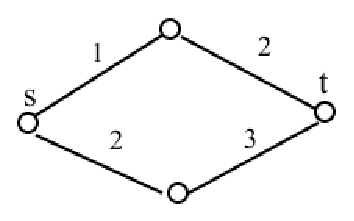
\includegraphics{initial_graph.eps}
	    \end{center}
	    \end{figure}

	      The algorithm will start with the weights vector being [1,1,1,1]. It will give the above graph and the weights vector as input to the 
	      ($\epsilon$, $\rho$)-oracle. For this example, let $\epsilon = \frac{1}{5}$ and let $\rho = \frac{3}{2}$. The oracle then constructs
	      a circuit as shown in the figure below, such that the values of resistances are as follows:
	      
	      
	      \begin{itemize}
	       \item 
		  $R_1 = (1 + \frac{1}{15}) = \frac{16}{15}$
		\item	
		  $R_2 = \frac{1}{4}(1 + \frac{1}{15}) = \frac{4}{15}$
		\item
		  $R_3 = \frac{1}{4}(1+\frac{1}{15}) = \frac{4}{15}$
		\item
		  $R_4 = \frac{1}{9}(1+\frac{1}{15}) = \frac{16}{135}$
	      \end{itemize}

	      \begin{figure}[htb]
		\begin{center}
		\leavevmode
		   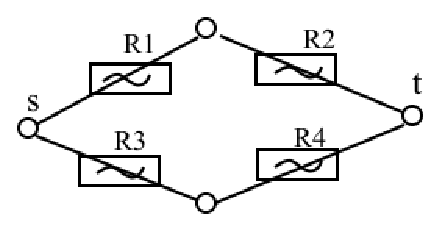
\includegraphics{resistance.eps}
		\end{center}
	    \end{figure}
	      
	      The oracle gives the above circuit with the resistance values as described, to the procedure that computes a $\delta$-approximate electrical
	      flow. Let the output flow by that procedure be [$\frac{5}{4}$, 1, $\frac{7}{4}$, 2]. It is easy to verify that this is infact an $\frac{\epsilon}{3}$
	      approximate electrical flow. \\
	      
	      Given this as the output, the weight update procedure updates the weights as follows
	      \begin{itemize}
	       \item 
		$w_1 = 1(1 + \frac{2}{15}(1+\frac{1}{4})) = \frac{7}{6}$
	      \item
		$w_2 = 1(1 + \frac{2}{15}) = \frac{17}{15}$
	      \item
		$w_3 = 1(1 + \frac{2}{15}(\frac{7}{8})) = \frac{67}{60}$
	      \item
		$w_4 = 1(1 + \frac{2}{15}) = \frac{17}{15}$
	      \end{itemize}
	      
	      With this new weights and the original graph and flow value of F=3, the algorithm again invokes the oracle. And a similar iteration happens.
	      This happens for about $N=150$ iterations, before the algorithm terminates. It takes the average of all the flows returned and multiplies
	      it by $\frac{8}{15}$. It returns this as the final flow vector.\\
	      
	      The simple example above illustrates the role of each procedure in the algorithm. \\
	    
	    \section{A $\widetilde{O}(m n^{\frac{1}{3}}\epsilon^{\frac{-11}{3}})$ time Flow Algorithm}
	      In this section, we continue to explain the algorithm proposed by \cite{DBLP:journals/corr/abs-1010-2921}. They use the previous algorithm as a base and further improve 
	      the running time. This improvement from the previous algorithm is achieved in two steps.
	      \begin{itemize}
	       \item 
		In the first step, by making some observations and hence modifying the updates procedure and the ($\epsilon, \rho$)-oracle, a
		$\widetilde(m^{\frac{4}{3}}\epsilon^{-3})$ algorithm is obtained.
	      \item
		 In the second step, the randomized sparsification method, as introduced by \cite{Benczur:1996:ASM:237814.237827}, is used to first 
		 sparsify the graph and then apply the algorithm which gives the required $\widetilde{O}(m n^{\frac{1}{3}}\epsilon^{\frac{-11}{3}})$
		 time flow algorithm.
	      \end{itemize}
	      
	      The key idea to execute the first step is to notice that, once an edge has been filled to capacity, it is better to remove it altogether
	      from the graph rather than assigning a large weight to it. This way the graph becomes smaller and smaller in subsequent iterations,
	      hence making the remaining steps faster. They call this set of edges removed as the forbidden edges. \\
	      
	      \begin{algorithm}[H]
	     \caption{A modified ($\epsilon, \rho$) - oracle}
	     \KwIn{
		\\
		Real number $F>0$ \\
		$w$ - vector of edge weights, where $w_e \geq 1 ~~ \forall e \in E$ \\
		set H of forbidden edges \\
	     }
	     \KwOut{
	      \\
	      A s-t flow $f$ satisfying the criteria and a set H' of forbidden edges. \\
	     
	     }
	     \Begin{
		- Set $\rho$ as $\frac{8m^{\frac{1}{3}}(\log m)^{\frac{1}{3}}}{\epsilon}$ \newline
		- Assign $r_e$ as $\frac{1}{u_e^2}\left( w_e + \frac{\epsilon \| w \| _1}{3m} \right)$ for each edge $e$ in the $E \setminus H$. \newline
		- Invoke Algorithm 4.1 using the above resistances and $\frac{\epsilon}{3}$ as the value of $\delta$.
		  Invoke it on the graph G(V, $E \setminus H$).\newline
		- Let $\overline{f}$ be the returned approximate electrical flow. \newline
		\uIf{$\epsilon_r(\overline{f}) > (1+\epsilon)\| w \| _1$ or s,t are disconnected on the set of edges $E \setminus H$}
		{
		    Return ``fail''
		 }
		 \uElseIf{$\exists~e$ with $cong_{\overline{f}}(e) > \rho$}
		 {
		    - Add all $e$ satisfying the condition $cong_{\overline{f}}(e) > \rho$ to the set H. \\
		    - Restart this procedure. \\
		 }
		 \lElse
		 {
		    Return $\overline{f}$
		 }
     
	     }
	    \end{algorithm}
	     As the reader would have observed, this just makes a small modification to the original oracle. It just ensures that those edges which have been
	     filled to capacity are eliminated from the graph. \\
	    	     
	     \begin{algorithm}[H]
	        \caption{A $\widetilde{O}(m^{\frac{4}{3}}\epsilon^{-3})$ time flow algorithm for maximum flow}
	        \KwIn{
		  \\
		  A graph $G$ \\
		  A vector u of edge capacities \\
		  A target flow value F \\
		  ($\epsilon, \rho)$ - oracle O \\
		}
		\KwOut{
		  \\
		  Either a flow $f$ or ``fail'' indicating $F > F^{\ast}$ \\
		}
		\Begin{
		  - Initialize the weights $w^0$ as $w_e =1$ for all the edges e. \newline
		  - Initialize H as $\phi$ \newline
		  - Initialize $\rho$ as $\frac{8 m^{\frac{1}{3}} \log^{\frac{1}{3}} m}{\epsilon}$ \newline
		  - Initialize N as $\frac{2\rho \ln(m)}{\epsilon^2}$ \newline
		  \For{i =1 to N}
		  {
		    - Query the oracle O with $w^{i-1}$, target flow as $F$ and the forbidden edge set as H \newline
		    \eIf{O returns a ``fail''}
		    {
			return ``fail''
		    
		    }
		    {
			 - Let $f^i$ be the value of the returned flow. \newline
			 - Replace H with the set $H'$ returned by the oracle. \newline
			 - Update weights as
			 $$w^{i} = w^{i-1}\ast\left(1+\frac{\epsilon\ast cong_{f^i}(e)}{\rho}\right)$$
		    }
		  }
		  - Return $f$ as $\frac{(1-\epsilon)^2}{(1+\epsilon)N}\left(\sum\limits_{i} f^i\right)$
		}
	      \end{algorithm}
	      
	      Similarly the main weights update procedure is modified to accommodate for the removal of forbidden edges. As it is already clear, the weights update
	      mechanism is untouched in this modified algorithm. Hence, our approach towards a parallel version can be easily adapted here. \\
	      
	      \subsection{Correctness and Running Time of the Modified Algorithm}
		
		The strategy to show the correctness is to prove a bound on u(H), which is the total capacity of the edges added to set H when the algorithm
		terminates. Also, the number of edges in set H is upperbounded at the end of the algorithm. More formally, the following theorem is proved. \\
		
		\begin{thm}
		  At the end of the algorithm, the following bounds hold true:
		  $$ \mid H \mid \leq \frac{30 m \log m}{\epsilon^2 \rho ^2} ~~~~~ and$$ 
		  $$ u(H) \leq \frac{30 m F \log m}{\epsilon^2 \rho ^3}$$
		  
		\end{thm}
		
		We will avoid the detailed proof of this theorem. The reader is advised to take a look at the proof given by \cite{DBLP:journals/corr/abs-1010-2921}. We will 
		just give the overall idea here. The key idea is to use the resistances of the network as potential function and note that edges
		that are added into H set are those that contribute to a significant fraction of the energy. Then, bound the maximum change in effective
		resistance during the run of the algorithm and hence bound H. \\
		
		Given this theorem, we will briefly show how the authors prove the running time. \\
		
		\begin{thm}
		  For $F \leq F^{\ast}$, the algorithm returns a flow $\overline{f}$, which is an (1-$\epsilon$)- approximation to F, in time
		  $\widetilde{O}(m^{\frac{4}{3}} \epsilon^{-3})$.
		\end{thm}
		
		\begin{proof}
		  The ($\epsilon, \rho$) - oracle either adds edges to the set H or makes a call to algorithm 4.1. The number of calls made to this 
		  algorithm is atmost N + $\mid H \mid$. And from theorem 8 we have an upper bound on $\mid H \mid$. Plugging this value and the 
		  value of N used, we get the required running time as 
		  (N + $\mid H \mid$)$\widetilde{O}(m \log(\frac{1}{\epsilon})) \leq \widetilde{O}(m^{\frac{4}{3}} \epsilon^{-3})$. \\
		  
		  Now, we need to show the part where it returns a flow $\overline{f}$, whenever $F \leq F^{\ast}$. \\
		  
		  Substitute the value $\rho$ used in the algorithm in theorem 8. We get,
		  $$u(H) \leq \frac{\epsilon F}{12}$$
		  
		  Hence, during the entire algorithm, the graph has a flow atleast $F^{\ast} - \frac{\epsilon F}{12} \geq (1-\frac{\epsilon}{12})F$.
		\end{proof}
		
		We will now show the step 2 by using the sparsification technique given by Karger et al. More formally, by direct application of the 
		following theorem given by them, we get the required improvement. 
		
		\begin{thm}
		 Given a T(m,n,$\epsilon$) algorithm to find a (1-$\epsilon$)-approximate flow in undirected graph, it can be used to obtain 
		 a (1-$\epsilon$)-approximate flow in time $\widetilde{O}(\frac{\epsilon^2 m}{n}T(\widetilde{O}(n \epsilon^{-2}),n,\epsilon))$ using 
		 ``graph smoothing'' as defined by Karger, et al.
		\end{thm}

		Hence, a direct application of this theorem with T(m,n,$\epsilon$) = $\widetilde{O}(m^{\frac{4}{3}} \epsilon^{-3})$ gives 
		the required bound of $\widetilde{O}(mn^{\frac{1}{3}} \epsilon^{\frac{-11}{3}})$. \\
		
		The drawback with using the above method of sparsification is that it is a probabilistic method. Hence, even though one can efficiently
		approximate the value of the flow, it is not possible to get a vector $f$ which is the approximation for this flow. This was an important
		open problem until recently \cite{DBLP:journals/corr/abs-1304-2338}, devised a different procedure that obtains a near linear time approximation for this
		problem which also gives the flow vector which approximates it. 
		
		\chapter{Future Directions and Important Open Problems}
		  In summary, we have done the following in this report. We first gave an exhaustive survey of all the classical algorithms that are known.
		  We then explained the CKMST algorithm in detail. We gave a procedure to generalize the weight updates. We then gave a baby-step
		  approach towards parallelism and finally gave some remarks as to why we believe this is a right direction. The main goal of our work
		  has been the following:
		  \begin{itemize}
		   \item 
		    Try and understand the nature of this problem and the previous work that researchers have done with regard to this problem.
		   \item
		    Try and answer one of the important open problems arising out of the CKMST algorithm - to give a parallel implementation of 
		    the algorithm.
		  \end{itemize}

		
		    The literature so far, has a collection of algorithms to compute the maximum flow in the graph. The CKMST algorithm broke 
		the running time barrier by introducing a bunch of newer techniques. Some of these techniques are applicable in other settings as well.
		In fact, this work has received a lot of attention in the recent past and is still far from completeness.
		There are a number of important questions arising out of this work. \\
		 
		 The following are some of the important open questions that are yet to be answered.
		 \begin{itemize}
		  \item 
		    As we have been trying in this work, it remains an open problem to make the CKMST algorithm completely parallel.
		    The advantage is that it can be used to compute the maximum flow on even larger graphs. It is also worthwhile to note that 
		 the newer algorithm that followed this by \cite{DBLP:journals/corr/abs-1304-2338} is also inherently sequential. Hence, it is currently an open problem to
		 to make the sequence of algorithms parallel. A first step towards this has been by \cite{DBLP:journals/corr/PengS13} where the authors have managed
		 to give a fully parallel solver for Laplacian systems. It must also be noted that all the classical algorithms are sequential
		 in nature and hence, parallelism has been a herculean task since the beginning.\\
		 
		 \item
		    Another important direction is devising a similar algorithm for directed graphs. The above algorithm looks at the graph as an electrical
		 circuit. By nature, resistors are bidirectional and hence, cannot be easily adapted in a directed graph setting. Getting an algorithm 
		 for directed graphs which runs in near linear time, will give a logical end to the sequence of sequential algorithms. \\
		 
		 \item
		    The current algorithm has a dependence of poly($\frac{1}{\epsilon}$) in its running time. It is interesting to make algorithms 
		 improve this bound and hopefully, bring the dependence down to poly($\log (\frac{1}{\epsilon})$). It should be noted that (1-$\epsilon$) is the approximation
		 ratio of the CKMST algorithm. The work by \cite{DBLP:journals/corr/abs-1304-2338} which followed this algorithm, also has a poly($\frac{1}{\epsilon}$)
		 dependence on $\epsilon$. Hence, devising algorithms(sequential or parallel) which makes this improvement is another important
		 direction researchers have been working in the recent times.
		 \end{itemize}
		 
		 
		
%%%%%%%%%%%%%%%%%%%%%%%%%%%%%%%%%%%%%%%%%%%%%%%%%%%%%%%%%%%%
% Bibliography.
\pagebreak
\begin{singlespace}
  \begin{small}
	\bibliography{refs}
  \end{small}
\end{singlespace}

%%%%%%%%%%%%%%%%%%%%%%%%%%%%%%%%%%%%%%%%%%%%%%%%%%%%%%%%%%%%

\end{document}
